\chapter{改进OpenShift Origin平台调度策略}
Kubernetes作为OpenShift Origin容器云平台的容器编排引擎,其默认配置的调度算法虽能满足大部分用户需求,但其算法较为简单,集群资源利用率较低,无法满足用户的在特定场景下的调度需求。本章在深入分析默认调度算法不足后,提出了一种新的基于多维空闲资源权重参数的评价函数和调度方案MRWS (Multidimensional Resource Weights Scheduling)。

\section{优化Kubernetes调度流程}
Kubernetes调度算法分为预选和优选两阶段,在预选阶段过滤掉不满足需求的节点,优选阶段对剩余节点评分,选择评分最高的节点作为调度目标。整个调度器可以分为待调度的Pod列表、满足条件的Node列表以及调度策略三部分。用户可以对其调度流程进行一定的优化,开发特定场景下的调度算法。

\subsection{Default调度算法流程}
在Kubernetes默认调度流程中,预选阶段解决节点过滤问题,优选阶段解决节点选择问题。用户可以对两个阶段进行简单的配置,调度器将根据用户指定的预选和优选规则进行过滤和评分计算,最终输出满足条件的Node和Pod绑定策略,将Pod调度到Node节点上,针对两阶段的规则,下面做详细的介绍。
\begin{figure}[H] % use float package if you want it here
	\centering
	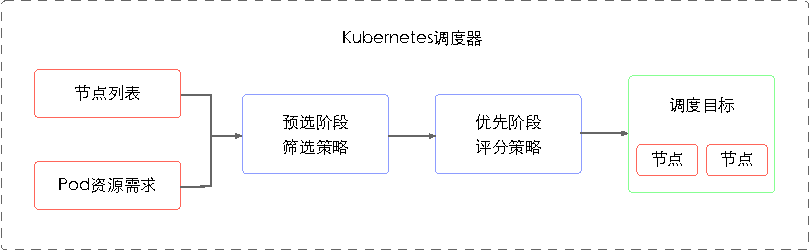
\includegraphics{scheduler-default}
	\caption{Default调度算法流程}
\end{figure}
Predicates阶段过滤掉不满足Pod资源需求的节点,依据一定规进行筛选,包括磁盘卷冲突、端口冲突、资源容量、节点检测、服务占用、亲和性等。1.7版本的筛选条件主要如下,新的版本Kubernetes正在不断完善和更新:
\begin{enumerate}[(1)]
	\item NoDiskConflict:检测卷冲突,在当前的规则中,两个不同Pod不能使用相同的卷。因此,一旦Node上挂载了该卷并被某个Pod使用,则新的Pod不能再调度到该Node上,否则造成卷冲突。不同的系统对该冲突检测范围不同,如Google Compute Engine在只读模式下允许多个卷,Ceph RDB允许两个Pod分享部分资源,Amazon EBS禁止两个Pod挂载同一个卷。
	\item NoVolumeZoneConflict:在给定Zone限制的条件下,检测Node上部署的Pod是否存在卷冲突,当前只限定对PV(Persistant Volume)范围进行支持。
	\item PodFitsHostPorts:端口冲突和服务占用检测,需要调度的Pod内所有的容器需要的端口在Node上是否被其他Pod占用。
	\item PodFitsResources:根据Pod资源的需求检测节点空闲资源量是否满足其运行需求,主要检测CPU、内存、磁盘等资源。Kubernetes的调度是静态调度,资源的判断是根据分配的资源量而不是资源的实际使用量。
	\item HostName:检测Pod是否指定了Node节点,所有不在指定Node集合内的节点都将被过滤掉。
	\item MatchNodeSelector:检测Pod是否指定了MatchNodeSelector属性,若指定了该属性,Node的Label必须和该属性匹配。
	\item MaxEBSVolumeCount:确保挂载的EBS存储卷总合不超过设置最大值,调度器计算每个Node上直接或间接使用的全部卷总合,一旦超过最大值,Pod不能调度到该节点上。
	\item CheckNodeMemoryPressure:判断节点是否存在内存压力,若存在内存压力则标记为1,Pod只能调度到内存标记为0的节点上。
	\item CheckNodeDiskPressure:判断节点是否存在磁盘压力,若存在磁盘压力则标记为1,Pod只能调度到磁盘标记为0节点。
	\item MatchInterPodAffinity:节点的亲和性过滤,检测Pod是否和已部署的Pod存在亲和性,将有亲和性的Pod调度到相同节点。
	\item PodToleratesNodeTaints:判断将Pod调度到节点后是否满足节点容忍的条件,相同的Pod副本为了满足容灾性,一般部署到不同的Node甚至是不同的机架和数据中心。
\end{enumerate}
此外、还有专为Google Compute Engine和Amazon EBS配置的MaxGCEPDVolumeCount、MaxAzureDiskVolumeCount卷检测条件,检测节点上挂载的卷容量总和是否超过了设定的最大值。

Priorities阶段根据一定的评分算法对预选出来的节点列表进行综合评分,评分依据主要包括资源空闲量、资源消耗平衡性、Pod亲和性、Pod与节点的匹配度等。Kubernetes使用优先函数集合内的函数对节点进行0-10评分,最终计算评分总和,评分越高表明Pod调度到该节点越适合,同时还可以为集合内的每一个函数设置一个权重值,主要的评分函数如下:
\begin{enumerate}[(1)]
	\item LeastRequestedPriority:、根据资源空闲率计算节点得分,即节点的空闲资源与节点资源总量的比值((节点资源总量-节点上Pod的资源和-新Pod的需求)/总容量)来计算。设置CPU和内存具有相同权重,都设置为0.5,资源空闲率越大,剩余资源越多,节点的评分就越高。
	\item BalancedResourceAllocation:该函数必须联合LeastRequestedPriority一起使用,用于平衡各项资源的使用率,资源使用越均衡,节点的评分越高。Kubernetes主要对内存和CPU资源消耗进行平衡,由两者的“距离”决定分值大小,即使用10-abs(CPU空闲率-内存空闲率)*10进行计算。
	\item SelectorSpreadPriority:为了更好应对容灾和宕机风险,同属Service、Replication Controller下的Pod尽可能分散部署到不同的Node上。对于指定Zone的Pod,也要尽量分散到不同区域的主机。调度器统计各Node上相同Service、Replication Controller下的Pod,Node上Pod数量越少,评分越高。
	\item NodeAffinityPriority:设置调度器的亲和性机制,主要对节点进行精确匹配。有两种选择器匹配模式,选择器“hard"模式下设置的NodeSelector必须和节点的Label匹配,保证选择的Node是完全满足需求规则的,”soft"模式下不能完全保证百分百的匹配,但会尽量满足规则要求
	\item ImageLocalityPriority:为避免镜像的重复下载对网络和磁盘资源的重复消耗,该函数根据Pod中运行容器需要的镜像对节点进行评分,节点上存在的镜像越多,该节点评分越高。若该节点上没有所需的镜像,评分为0,镜像评分的权重可以根据镜像大小按比例决定。
	\item MostRequestedPriority:和LeastRequestedPriority相反,两者使用一个来计算评分。该函数确保使用资源越多的节点,评分越高,目的在于使用更少的服务器提供服务,节约集群资源,提升资源利用率。
	\item TaintTolerationPriority:容忍性评分函数,匹配Pod的TolerationList与节点Taint,匹配项越多,该节点的容忍性越好,从而评分越高。
	\item InterPodAffinityPriority:用于迭代WeightedPodAffinityTerm的元素计算和,若该节点同时满足亲和性设置,则将该评分加入节点的整体评分中。
	\item NodePreferAvoidPodsPriority:根据节点是否设置Anotation属性进行评分,没有设置该属性则评分为10,设置该属性并且调度的Pod正好是副本,则该节点评分为0,目的在于避免相同副本调度到同一节点。
\end{enumerate}

优先调度模块定义了一个评分函数集合,各评分函数的权重可以指定,用户根据调度依据的重要程度给各函数赋予不同的权重值,最终所有函数的评分总和就是该节点的最终得分,选择评分最高的节点作为Pod的调度目标。

\subsection{MRWS算法调度流程}
Kubernetes调度系统的Default算法核心在于优选阶段的评分函数,调度策略根据节点评分高低做出调度决策。在所有的评分函数中,除一些特殊的调度规则外,如节点亲和性、节点容忍度、节点上的镜像文件等,最为重要的是根据资源空闲率做出评分的LeastRequestedPriority和资源使用平衡性做出评分的BalancedResourceAllocation函数。这两个函数是整个评分函数集合中的核心,在其他外在规则相同的条件下,直接决定节点的评分高低。但是,这两个评分函数仅考虑了内存和CPU的空闲率和消耗平衡性,这种评分会造成节点其他维度资源消耗不均,如磁盘、网络带宽、节点上运行的Pod数量等。一旦某个维度的资源过载,节点将不能部署更多的Pod,造成集群资源利用率低下。因此,新的调度算法MRWS将综合考虑集群CPU、内存、磁盘、网络带宽以及节点运行Pod数量的均衡性,提升集群的负载均衡和资源利用率。
\begin{figure}[H] % use float package if you want it here
	\centering
	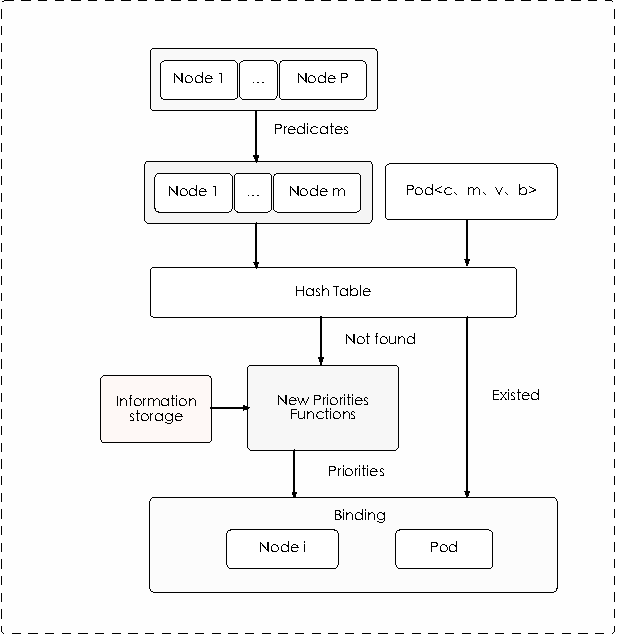
\includegraphics{scheduler-mrws}
	\caption{MRWS算法调度流程}
\end{figure}
在Default算法中,优选阶段根据评分集合进行节点评分,其评分函数如下:
\begin{equation}
	S_{i} = (w_{1}*f_{1})+(w_{2}*f_{2})+...+(w_{jj}*f_{j})+...(w_{p}*f_{p})
\end{equation}
其中,\begin{math}S_{i}\end{math}是第i个节点的总评分,\begin{math}w_{j}\end{math}是第j个评分函数权重,\begin{math}f_{j}\end{math}是第j个评分函数,每个函数的权重可以根据用户的需求进行指定。

如图3.2所示,新的调度算法MRWS首先对调度流程进行优化,预选阶段从集群上的\emph{P}个节点中根据预选规则选出\emph{M}个节点,这些节点满足Pod调度的资源需求和预先设定的筛选条件。\emph{M}个节点列表和Pod的内存、CPU、磁盘、带宽需求作为评分阶段的输入,查找Hash表中该Pod以前是否被创建和调度过,若该Pod之前被调度过并且以前调度的节点同时在预选阶段剩余的节点中,将新Pod直接绑定到节点。通过Hash表的作用,可以避免重复的Pod被调度到不同的节点,导致容器镜像被重复下载,节约磁盘空间和网络资源,缩短Pod应用的调度算法计算时间,使集群具有调度记忆功能。若Pod是一个新建的Pod,进入函数评分模块,信息存储模块通过节点上的cAdvisor资源监控代理收集集群整个资源,同时记录各节点上已分配的Pod资源总量和Pod运行数量,权重参数库存储容器应用资源权重系数。最终通过全新的评分函数体系进行节点评分,该评分函数核心在于对节点资源建模,通过数学方法FAHP自动求解其参数,使集群中各节点各维度资源利用更加均衡。

\section{MRWS调度算法设计}
Kubernetes调度器评分阶段的核心算法仅考虑内存和CPU空闲率以及消耗平衡性,容易造成其他维度资源过载,从而使集群资源利用率低下。MRWS算法将综合考虑集群节点的CPU、内存、磁盘、网络带宽以及节点上已运行的Pod数量等因素,致力于多维资源的均衡利用,尤其是在大数据处理多计算框架同时部署的场景下,让各计算框架的应用调度更加合理,缩短应用的执行时间。整个MRWS算法分为资源空闲率评分模块,平衡评分模块和算法均衡度评价模块三部分,下面分别对其建模和计算方法进行详细介绍。

\subsection{MRWS空闲资源评分}
为了达到集群多维资源利用均衡,提升集群服务性能的目的,某个节点空闲资源越多并且各维度消耗越平均,该节点的评分就应该越高,就越适合新创建Pod节点的部署。针对大规模的集群,每个节点资源消耗均衡性不能完全依赖人为判断,并且评分函数的权重参数也不能全部由人工赋予,这种方式既不科学也不准确。用户应用场景和对资源重要性判断的差异性,将导致相同应用在同一调度算法下的不同调度结果。为了避免此种情况发生,需要对预选阶段剩余的节点建模,使用一定数学方法对资源的权重参数自动求解。在构建评分算法前,先对集群节点和Pod资源需求进行建模(建模中节点是预选阶段过滤后的节点):
\begin{enumerate}[(1)]
	\item 定义集群节点和资源的符号表示。假设\emph{P}个节点列表经过预选阶段筛选后剩余\emph{M}个节点,表示为\begin{math}N=(n_{1}, n_{2}, n_{3}...n_{m})\end{math}。单个节点的资源维度为\emph{D},在该模型中考虑节点CPU、内存、磁盘和网络带宽四种资源因素,因此\emph{D}=4。集群中单个节点的资源总量表示为\begin{math}S=(s^{d}_{1}, s^{d}_{2}, s^{d}_{3}...s^{d}_{m}),\quad d\in{D}\end{math},其中\begin{math}s^{d}_{i}\end{math}表示第i个节点拥有的第d维资源的总量。同理,可以定义节点各维度资源的使用量,表示为\begin{math}R=(r^{d}_{1}, r^{d}_{2}, r^{d}_{3}...s^{d}_{m}),\quad d\in{D}\end{math},其中\begin{math}r^{d}_{i}\end{math}表示第i个节点上第d维资源的使用量。当前需要调度的Pod对资源的需求可以表示为\begin{math}p^{d},\quad d\in{D}\end{math},表示Pod对d维度资源的需求量。
	\item 已部署Pod空闲率计算。节点上已部署Pod应用数量可以记录和统计,但将其作为影响调度策略的因素时没法加以限制和度量,也不能指定节点部署Pod总量。针对已部署Pod这个影响调度的因素,需要单独进行处理,使用一定的方式计算其负载和资源空闲率。考虑该因素的目的在于使每个节点部署的Pod数量尽量接近,若某个节点部署少量大资源需求的Pod,另一个节点部署大量小资源需求的Pod,虽然两个节点资源使用率相近,但是大量小资源数量Pod的管理会极大增加节点开销,影响该节点的服务质量。因此,应尽量使不同节点上运行的Pod数量均衡。采用如下的方式计算节点已部署Pod的负载,集群中预选阶段剩余节点上已调度的Pod总数C表示为:
	\begin{equation}
	C = (\sum_{i=1}^{m}p_{i} + 1)
	\end{equation}
	其中,\begin{math}p_{i}\end{math}表示第i个节点上已部署的Pod数量,可以用$c_{i}$表示第i个节点已部署Pod的资源空闲率,如式(3-3)所示。
	\begin{equation}
	c_{i} = (1-\frac{p_{i}+1}{C})
	\end{equation}
	\item 多维资源的权重系数。在评分函数模块,给评分函数集合中的每个评分函数人为赋予一个权重,最终按照总得分排名选取最高。在实际的数据中心中,根据用户调度Pod请求的资源数量可以感知部署的应用类型,如CPU密集、内存密集、I/O密集以及网络密集型等。从经济效益角度考虑,节点上各种资源重要程度也具有较大差异,CPU和内存较为稀缺,价格相对昂贵一点。定义权重系数\begin{math}\alpha_{i}(i=1, 2, 3, 4, 5)\end{math}分别用于表示节点CPU、内存、磁盘I/O、网络带宽和已部署Pod数量等因素的重要程度,且$\alpha_{1}+\alpha_{2}+\alpha_{3}+\alpha_{4}+\alpha_{5}=1$。权重参数将在下一章通过FAHP进行节点资源数学建模并实现自动求解,用户通过微调权重参数更加灵活使用新调度算法。
\end{enumerate}

根据上述定义的集群符号,可以根据各节点资源空闲率对节点进行评分,资源空闲率模块反映节点空闲资源的数量,空闲资源越多,节点评分越高。在考虑资源空闲量时又充分考虑各维度资源的重要程度,越是宝贵的资源其重要程度越高。节点i空闲模块的最终评分$v_{i}$如式(3-4)所示。
\begin{eqnarray}
v_{i} & = & \sum_{d=1}^{D}\alpha_{d}*k_{i}^{d}+\alpha_{5}*c_{i} \\[0.3cm]
k_{i}^{d} & = & \frac{s_{i}^{d}-r_{i}^{d}-p^{d}}{s_{i}^{d}}
\end{eqnarray}
其中,$k_{i}^{d}$表示节点i部署$p^{d}$后第d维资源的空闲率。

\subsection{MRWS平衡模块评分}
在空闲资源模块评分中,各个维度的资源通过其空闲量和资源的重要程度影响评分,这会导致各维度资源利用不均衡。比如某个节点CPU资源空闲率很低,但其他维度空闲率很高,尽管赋予了CPU较高影响因子\begin{math}\alpha_{1}\end{math},但其整体评分依然偏高,会继续调度CPU密集的Pod到该节点,造成节点性能下降,资源消耗更加不均衡。为避免上述情况的发生,需要设计一个平衡模块,用于平衡各维度资源消耗。平衡模块用于反映节点各维度资源的均衡状况,各维度资源消耗越均衡,其评分越高。计算预选阶段剩余节点各维度资源空闲率的均值如式(3-5)、(3-6)所示。
\begin{eqnarray}
k_{v}^{d} &=& \frac{(\sum_{i=1}^{m}k_{i}^{d})}{m} \\[0.3cm]
c_{v} &=& \frac{(\sum_{i=1}^{m}c_{i})}{m}
\end{eqnarray}
其中,\begin{math}k_{v}^{d}\end{math}表示经预选阶段筛选后剩余m个节点上第d维资源空闲率的平均值,\begin{math}c_{v}\end{math}表示剩余节点上已部署Pod资源空闲率的平均值。因此,可以使用\begin{math}(1-\left |k_{i}^{d}-k_{v}^{d}\right |)\end{math}来度量节点i上第d维资源空闲率在集群中的不均衡性。同理,\begin{math}(1-\left |c_{i}-c_{v}\right|)\end{math}
表示节点已部署Pod数量的不均衡性。该值越大,表明各维度资源利用越均衡,节点评分越高。平衡模块节点的最终评分\begin{math}b_{i}\end{math}如式(3-8)所示。
\begin{equation}
b_{i} = \frac{\sum_{d=1}^{D}(\alpha_{d}(1-\left |k_{i}^{d}-k_{v}^{d}\right|)+\alpha_{5}(1-\left |c_{i}-c_{v}\right|))}{D+1}
\end{equation}

整个评分算法综合考虑CPU、内存、磁盘、网络带宽以及已部署Pod等因素,分值由资源空闲评分和资源均衡评分组成。资源空闲率反映节点可用资源的状况,资源均衡反映节点各维度资源消耗的均衡性,单个节点最终评分如式(3-9)所示。
\begin{equation}
f_{i} = v_{i}+b_{i}
\end{equation}

\subsection{MRWS均衡度评价模块}
设计完调度算法后需要对调度算法多维资源利用均衡性进行度量,由于资源重要程度不同,不能简单用空闲资源利用率总合进行加权平均计算。在概率论和统计中,通常用方差来度量一组数据的离散程度,计算一个变量与整体均值之间的差异。因此,用预选阶段剩余节点的多维资源空闲率的方差来度量集群的负载均衡性,定义集群的负载均衡度$u_{v}$如式(3-11)。
\begin{eqnarray}
	u_{i} &=& \sqrt{\frac{1}{D+1}(\sum_{d=1}^{D}(k_{i}^{d}-k_{v}^{d})^{2}+(c_{i}-c_{v})^{2})} \\[0.3cm]
	u_{v} &=& (\sum_{i=1}^{m}u_{i})/m
\end{eqnarray}
其中,\begin{math}u_{i}\end{math}表示节点i上多维资源空闲率的负载均衡,该值越小,表示多维资源利用越均衡,即各维度资源利用越接近平均值。因此,用集群中满足预选阶段剩余节点负载均衡的均值表示集群的负载均衡度。这种使用方差度量集群均衡性的方法不仅适用于MRWS算法,对于Kubernetes默认的Default算法以及Random、FirstFit算法同样适用。在后面进行算法性能对比实验中,将使用上式的负载均衡度衡量不同调度算法下集群的负载均衡性。

\section{本章小结}
本章首先详细介绍OpenShift Origin容器云平台的容器编排引擎Kubernetes的默认调度算法Default的调度流程,该流程分为预选和优选两个阶段。接着对预选阶段的筛选规则和优选阶段的评分函数集合进行分析。针对其调度流程和调度算法的不足,提出了一种MRWS调度算法,该算法先对调度流程进行适当的优化,使其调度记忆功能。然后根据算法的需要对集群和应用资源建模,转为为数学表示,为下一章使用FAHP权重参数求解打下基础。最后设计了详细的评分规则,根据权重参数和资源的乘积和进行评分计算,资源的权重参数自动求解将在下一章节进行详细的介绍。




